\section{Introduction}

% The Cookie Theft is a picture widely used in diagnosing human language and cognitive abilities.
% It is from the Boston Diagnostic Aphasia Examination~\cite{goodglass2001-ej} first published in 1972. 
% To this day, this picture is still widely used.
% \MY{How complexed a picture can be? What kind of story can be told via a single picture? As the saying goes, ``a picture is worth a thousand words''. However, not every picture contains such rich information.}
How complex can a picture be?
What kind of story can be told via a single picture? 
As the saying goes, ``a picture is worth a thousand words''. 
However, not every picture contains such rich information.
The ``Cookie Theft'' (Figure~\ref{ct} (a)) is a good exemplar for complex semantic information expressed via visual language. 
% \MY{i revised this sentence, pls check}
It is a well-known picture commonly used to assess language and cognitive abilities in humans. 
It was first introduced in the Boston Diagnostic Aphasia Examination published in 1972~\cite{goodglass2001-ej} and remains widely utilized to this day.

Many studies~\cite{cummings2019describing, tasnim-etal-2022-depac} have revealed the reasons behind the success of this picture.
Its essence is being a ``good storyteller,'' capable of telling a complete and engaging story. 
% Specifically, two of its most important features are\MY{say something like psychologists summarized the two most important features}: 
Based on the research of the psychologists, two of its most important characteristics can be summarized as follows: 
(1). It contains a rich but not excessive number of entities, making it well-suited for eliciting longer narrative descriptions. 
(2). It is rich in semantics, enabling it to tell an interesting story.
The semantics are derived from reasonings made by observing the entities and their relationships in the image.
For instance, the Cookie Theft tells a story about two children attempting to steal cookies from a jar when their mother is not looking. 
The mother-child relationship between the characters in the image is deduced through further reasoning based on observing the content in the image.

% \begin{figure}[htbp]
%     \centering
%     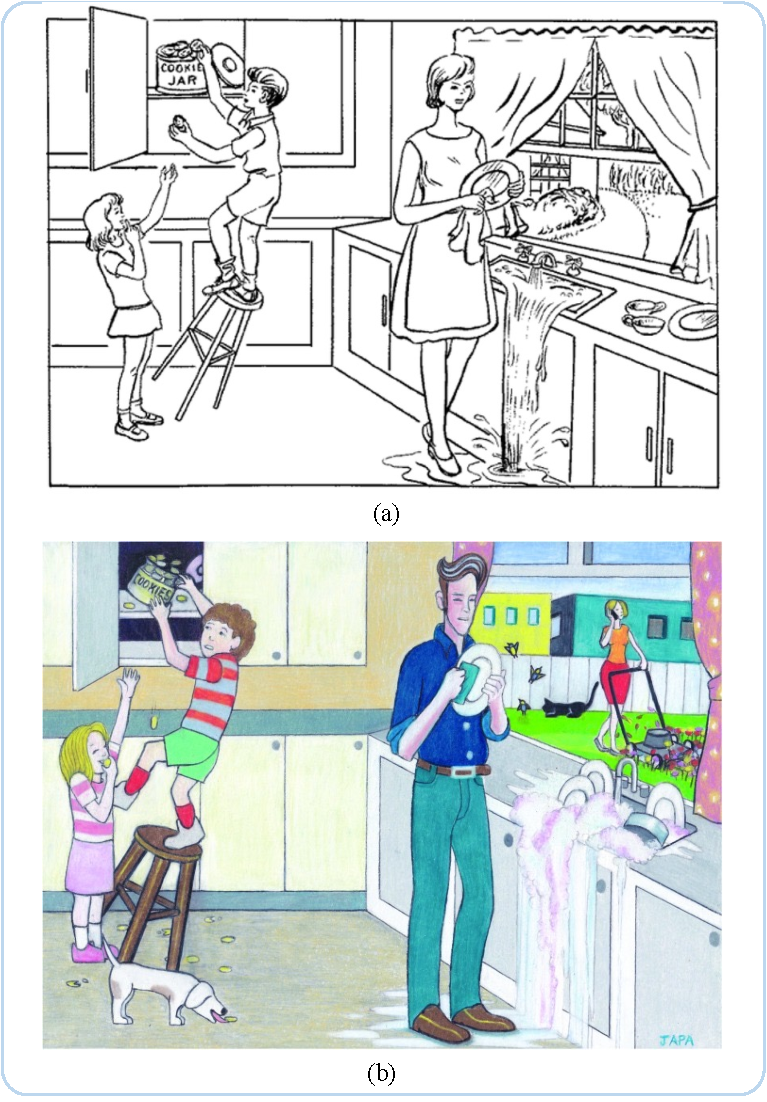
\includegraphics[scale=0.38]{figs/cookie_theft2.pdf}
%     \caption{The Cookie Theft pictures. (a) is the original version and (b) is the updated version.}
%     \label{ct}
% \end{figure}

\begin{figure}[htbp]
    \centering
    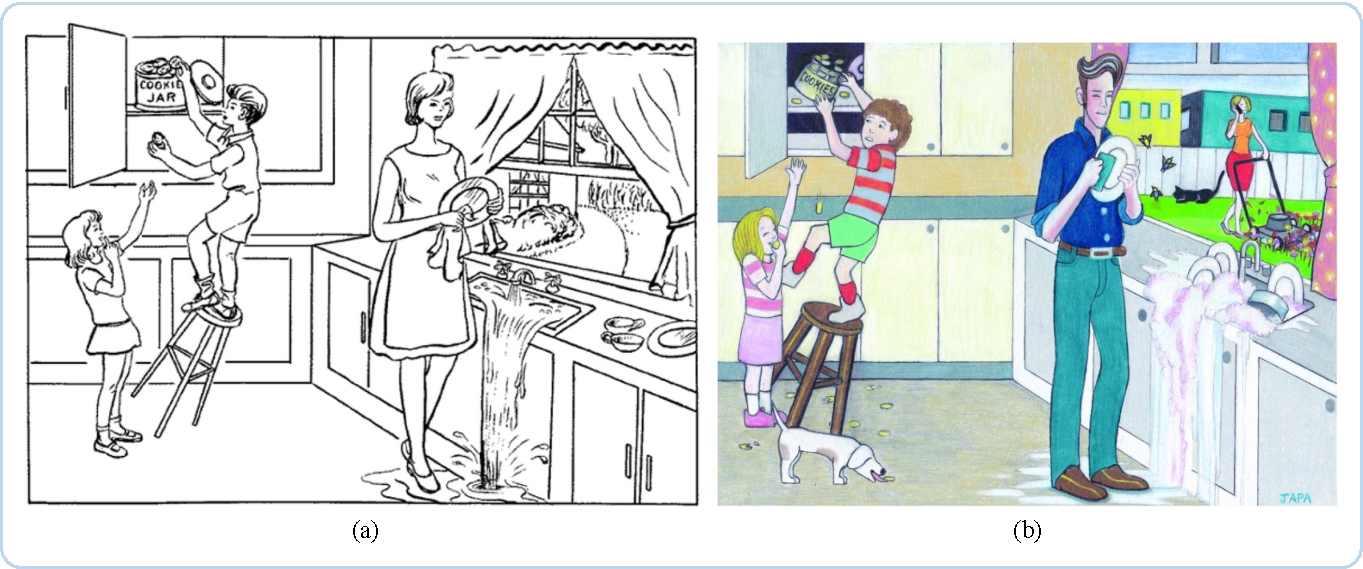
\includegraphics[scale=0.36]{figs/cookie_theft3.pdf}
    \caption{The Cookie Theft pictures. (a) is the original version and (b) is the updated version.}
    \label{ct}
\end{figure}


% A mother who is drying dishes next to the sink in the kitchen. 
% She is not paying attention and has left the tap on. 
% As a result, water is overflowing from the sink. 
% Meanwhile, two children are attempting to take cookies from a jar when their mother is not looking. 
% One of the children, a boy, has climbed onto a stool to get up to the cupboard where the cookie jar is stored. 
% The stool is rocking precariously. 
% The other child, a girl, is standing next to the stool and has her hand outstretched ready to be given cookies.

Though the Cookie Theft picture is widely used, there are still limitations. 
It is outdated since it has been proposed for half a century and it cannot be well applied to different cultures~\cite{berube2019stealing, rethinkingct}.
To avoid these issues, people often have to modify or replace the image in different application scenarios~\cite{berube2019stealing, HUSSEIN2015152, DOMINGUEZ2006476, Oh2012ValidityAR, Prasad2012ValidationOT}.
For instance, Figure~\ref{ct} (b) is an updated version of the Cookie Theft.
This means more images of this kind are necessary. 
% \KZ{I think this para can be expanded a bit more: also talk about using the same pic repeated on the same patient doesn't work well.}

Besides, this kind of image is not only useful for humans but also for Artificial Intelligence (AI).
With the development of vision models, especially Large Vision-Language Models (LVLMs), their abilities are increasing rapidly. 
% \KZ{It's not clear to me why more images like the cookie theft pic can improve these AI models. Improve their cognitive ability? Or is it for evaluating these AI models?}
Simple images with less semantics are not challenging enough for them anymore, so more images with rich semantics will definitely be beneficial for both training and evaluation~\cite{song2024cognitive}.

% Considering the two motivations above, it is necessary to retrieve more storytelling images with rich semantics.
The internet or existing image datasets contain a lot of images, including some high-quality images that we want. 
% However, due to the scarcity of such high-quality images, locating or identifying them from a large pool of images is challenging.\MY{However, due to their scarcity, identifying and locating these high-quality images amidst the vast array of webly images can be a daunting task. Therefore, efficient methods for scoring and selecting these images are crucial.}
However, due to their scarcity, identifying and locating these high-quality images amidst the vast array of webly images can be a daunting task. 
Therefore, efficient methods for scoring and selecting these images are crucial.
% \KZ{Retrieve from where? I think you need to say that the WWW contains a lot of images, including these ``good'' images that we want. But they maybe sparse, so locating or identifying them from a large pool of image is the challendge?}
% However, this kind of images are rare and it is challenging to find this kind of images. 
% Thus, how to effectively find this kind of images is important.
% However, this kind of images are rare and challenging to locate. 
% finding an effective way to identify them
% Therefore, it is crucial to automatically evaluate semantic complexity in an image.\MY{consider deleting this first sentence as I just included in my previous comment}
It can not only tell us how suitable an image is to assess cognitive capability as ``Cookie Theft'', but also retrieve high-quality images for AI training and evaluation.
Furthermore, with the advancement of image generation models~\cite{Rombach2021HighResolutionIS, pmlr-v139-ramesh21a, Ramesh2022HierarchicalTI}, they are also increasingly capable of helping us generate more and more images.
Thus, automatic semantic complexity assessment can also be used to guide the image generation task. 

Currently, though there are some research works about Image Assessment, like Image Quality Assessment (IQA)~\cite{Fang_2020_CVPR, ying2020patches}, Image Aesthetics Assessment (IAA)~\cite{ijcai2022p132, Yi_2023_CVPR}, and Image Complexity Assessment (ICA)~\cite{saraee2020visual, ic9600}, no one focuses on assessing the semantic complexity of images.
In order to fill this research blank, we propose the \textbf{Image Semantic Assessment (ISA)} task to assess the semantic complexity of images.

% As we mentioned above, this kind of images should have not only rich entities, but also rich semantics. 
% For example, though images with abundant entities are preferred for cognitive test, it does not mean more is always better.
Considering entities are the foundation of semantics and the complexity requirements for these two aspects may vary in different application scenarios, ISA task assesses images from both two levels: 
1) At the \textbf{\textit{entity}} level, we mainly adopt the idea of ICA task~\cite{ic9600}, assessing the entity richness of images, which we refer to as the Entity Complexity Scoring task; 
2) At the \textbf{\textit{semantic}} level, we propose the Semantic Complexity Scoring task to assess the higher-level semantic complexity of images. Note that this sub-task is the core of our proposed ISA task.
% which is .

To promote the research on ISA task, we built the first ISA dataset with 2,340 images.
Each image is annotated with the two corresponding scores by three annotators.
Besides, a corresponding method called \textbf{V}ision-\textbf{L}anguage collaborative \textbf{ISA} method (\textbf{VLISA}) is proposed for this novel task. 
It first uses a Large Vision-Language Models (LVLM), such as GPT-4o, as a feature extractor to extract semantic information in natural language form from images. 
Then, a regression model is trained to predict the score of images.
Our contributions are as follows:

1. As far as we know, we are the first to propose the ISA task, which aims to automatically assess semantic complexity in an image. 
It can be used to find higher-quality images with rich semantics and evaluate image generation models etc. 

2. We construct the first ISA dataset consisting of 2,340 images and human scores that supporting the ISA task. Our dataset includes images of varying semantic complexity, which helps models learn the ability to assess semantic complexity.

3. To effectively assess the semantic complexity of images, we propose a simple yet effective method that collaboratively utilizes language and visual information.
% \MY{that collaboratively utilizes language and visual information}.
Experiments show that ISA task is challenging for traditional vision models like ViT and our proposed method significantly outperforms other baseline models on the Semantic Complexity Scoring task.
% \KZ{Weak!}
 % our proposed VLISA can effectively score the semantic richness of images.